\subsection{Dot Product}

You may have noticed that while we can add and subtract vectors, and we can multiply them by scalars, there is no allowance for multiplying or dividing two vectors. In general, there is no requirement for a well-defined product of two vectors in a vector space. However, there are a couple of useful ``product" operations that show up with real-valued vectors. One of these is called the \textbf{dot product}.

\begin{definition}{Definition of Dot Product}
Let $\vcv$ and $\vcw$ be two vectors in $\bbr^n$. Then the \textbf{dot product} of $\vcv$ and $\vcw$ is defined as:
\begin{align*}
\vcv\bullet\vcw=&\sum_{i=1}^n v_i w_i \\
=&v_1 w_1 + v_2 w_2 +\cdots+v_n w_n 
\end{align*}
\end{definition}

\begin{exercise}{}
Find the following dot products:
\begin{enumerate}
\item $(3,2)\bullet(2,7)$
\vspace{1em}
\item $(1,2,3)\bullet(-2,3,1) $
\vspace{1em}
\item $(2,6,-4,-1)\bullet(-1,3,-4,2)$
\vspace{1em}
\item $(3,-14,12)\bullet(-24,21,3)$
\vspace{1em}
\end{enumerate}
\end{exercise}

% The vector drawn from the starting point to the ending point is exactly the sum of the two vectors. The difference of two vectors can be found from the same triangle as the sum:

% \begin{center}
% \begin{tikzpicture}[scale=.7, x=1cm, y=1cm, semitransparent]
% 	%\draw[step=1mm, line width=0.1mm, black!20!white] (0,0) grid (\width,\hauteur);
% 	%\draw[step=5mm, line width=0.2mm, black!90!white] (0,0) grid (\width,\hauteur);
% 	\draw[step=5cm, line width=0.5mm, black!90!white] (0,0) grid (\width,\hauteur);
% 	\draw[step=1cm, line width=0.2mm, black!50!white] (0,0) grid (\width,\hauteur);
% 	\draw[->, color=blue,line width=0.5mm](5,5)--(7.6,6);
% 	\node[color=blue] (v) at (6,6){$\vcv$};
% 	\draw[->, color=red, line width=0.5mm](5,5)--(7,3.6);
% 	\node[color=red] (u) at (5.6,3.8){$\vcu$};
% 	\draw[->, color=violet, line width=0.5mm](7.6,6)--(7,3.6);
% 	\node[color=violet] (w) at (7.8,4.5){$\vcw$};
% 	\end{tikzpicture}\end{center}

% Here, $\vcv+\vcw=\vcu$. Then it follows that $\vcu-\vcv=\vcw$. That is, the difference between two vectors is the vector that goes from the tip of the second (``negative") vector to the tip of the second (``positive") vector.

\begin{exercise}{The Law of Cosines and the Dot Product}
Sometimes, given two vectors $\vcv=(v_1,v_2)$, $\vcw=(w_1,w_2)$ with angle $\theta$ between them the expression $$\vcv\bullet\vcw=||\vcv|| \ ||\vcw||\cos\theta. $$ is referred to as ``the dot product version of the law of cosines". Why? Let's find out. We'll start by constructing a vector triangle, placing $\vcv$ and $\vcw$ in standard position:
\begin{center}
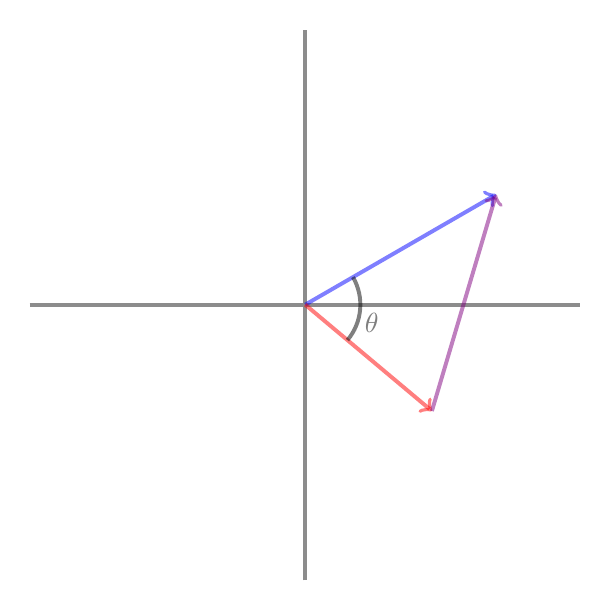
\begin{tikzpicture}[scale=.7, x=1cm, y=1cm, semitransparent]
	%\draw[step=1mm, line width=0.1mm, black!20!white] (0,0) grid (\width,\hauteur);
	%\draw[step=5mm, line width=0.2mm, black!90!white] (0,0) grid (\width,\hauteur);
	\draw[step=5cm, line width=0.5mm, black!90!white] (-5,-5) grid (4.99,4.99);
	%\draw[step=1cm, line width=0.2mm, black!50!white] (-5,-5) grid (5,5);
	\draw[->, color=blue,line width=0.5mm](0,0)--(30:4);
	\node[color=blue] (v) at (1.25,1.5){$\vcv$};
	\draw[->, color=red, line width=0.5mm](0,0)--(320:3);
	\node[color=red] (u) at (.75,-1.25){$\vcw$};
	\draw[->, color=violet, line width=0.5mm](320:3)--(30:4);
        \draw[line width=0.5mm] (320:1) arc (-40:30:1);
        \node (theta) at (-15:1.25){$\theta$};
	%\node[color=violet] (w) at (7.8,4.5){$\vcw$};
	\end{tikzpicture}\end{center}
	\begin{itemize}
	\item What is the purple vector (from the tip of $\vcw$ to the tip of $\vcv$)? Hint: Think about the geometric difference of two vectors.
	\vspace{5em}
	\item What are the lengths of the three sides of this triangle? Hint: The length of a vector is its \textbf{magnitude}.
	\vspace{5em}
	\item Using the Law of Cosines, write an expression relating your three side lengths and $\theta$.
	\vspace{10em}
	\item Show that this expression simplifies to $$\vcv\bullet\vcw=||\vcv|| \ ||\vcw||\cos\theta. $$
	Hint: Leave $-2||\vcv|| \ ||\vcw||\cos\theta$ alone for now, but expand out all of the other magnitudes using the magnitude formula, expand, then see if anything cancels.
	\vspace{50em}
	\end{itemize}
\end{exercise}

Note that this rule $$\vcv\bullet\vcw=||\vcv|| \ ||\vcw||\cos\theta$$ does \textit{not} just hold in $\bbr^2$ but in all $\bbr^n$. So in fact, the dot product can be used to identify the angle between two given vectors in any $\bbr^n$. This is particularly useful when we're deciding if two vectors are \textbf{orthogonal}, that is, if they have an angle of $90^\circ$ between them.

\begin{exercise}{}
Use the dot product to find the following angles.
\begin{enumerate}
\item Let $\vcv=2\vci+2\vcj$ and let $\vcu=-\vci+\vcj$. Find the angle between $\vcv$ and $\vcu$.
\vspace{1em}
\item Let $\vcv=\bmat{3\\2\\1}$ and let $\vcu=\bmat{2\\-5\\1}$. Find the angle between $\vcv$ and $\vcu$.
\vspace{1em}
\end{enumerate}
\end{exercise}
